\section{Architettura del prodotto}

\subsection{Architettura logica}
Il sistema \capName\ consiste di uno \textit{smart contract} per gestire i pagamenti e le recensioni, e di una \textit{web app} che permette l'interazione con esso tramite il \textit{wallet} \textit{MetaMask}. È anche presente un servizio \textit{API REST} che permette agli \textit{e-commerce} interessati di accedere alle recensioni per facilitarne l'integrazione nel loro sito web.

La web app interagisce direttamente con la \textit{blockchain} tramite \textit{Remote Procedure Call} utilizzando un nodo per dialogare con lo smart contract. D'altra parte, il servizio \textit{API REST} è separato dalla logica dell'applicazione e ha come unico scopo quello di fornire un'interfaccia standard e facile da usare per gli \textit{e-commerce}, che permette loro di visualizzare le recensioni sul proprio sito.

\subsection{Architettura di deployment}
L'architettura di \textit{deployment} del prodotto prevede la suddivisione dei componenti in tre nodi distinti:
\begin{itemize}
    \item \textit{Server web app}: ospita la \textit{web app} e comunica con lo \textit{smart contract} attraverso l'utilizzo della libreria \texttt{web3js};
    \item \textit{Server API}: ospita l'\textit{API REST} e comunica con il \textit{smart contract} attraverso l'utilizzo della libreria \texttt{web3j};
    \item \textit{Nodo Ethereum}: nodo per dialogare direttamente com la blockchain \textit{Ethereum} tramite \textit{Remote Procedure Call}. È utilizzato sia dal \textit{server web app} che dal \textit{server API}. Fornito da \textit{Infura}.
\end{itemize}
\pagebreak

\subsection{Dettaglio architettura}
\subsubsection{Smart contract}

Lo \textit{smart contract} è stato sviluppato in \textit{Solidity} e pubblicato su \textit{Sepolia}, una \textit{testnet} di \textit{Ethereum}, per permettere la verifica del suo funzionamento.

\paragraph{Diagramma delle classi}~
\begin{figure}[H]
    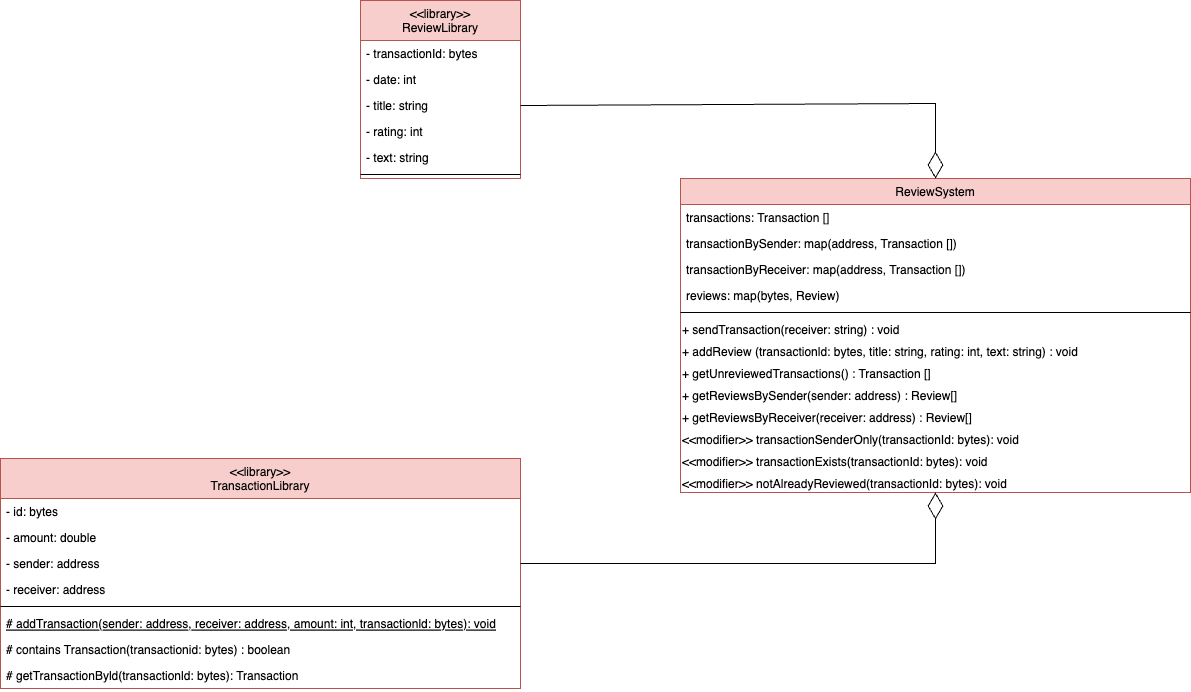
\includegraphics[width=\linewidth]{src/img/contract.png}
    \caption{Diagramma delle classi dello \textit{smart contract}}\label{fig:contract}
\end{figure}
\subparagraph*{Commento sui \texttt{modifier}}~

\noindent In \textit{Solidity} le funzioni possono essere modificate da particolari \texttt{modifier}, che permettono di aggiungere delle condizioni che devono essere verificate prima dell'esecuzione della funzione. Questi sono stati inseriti nel diagramma come delle funzioni private con tipo di ritorno nullo.

\paragraph{Design patterns}~
\subparagraph*{Access Restriction}~

\noindent Limita la chiamata di alcune funzioni ad una ristretta tipologia di utenti.

Viene utilizzato per limitare la possibilità di rilasciare una recensione per una determinata transazione solo all'effettivo cliente che l'ha effettuata. Avviene tramite \texttt{modifier} del linguaggio, particolari funzioni che permettono di bloccare l'esecuzione della funzione a cui vengono legati e annullare l'operazione se non viene rispettata la condizione.

\subparagraph*{Guard check}~

\noindent Valida i parametri passati ad una funzione, annullandola se non rispettano determinate condizioni.

Tramite \texttt{require}, un meccanismo di validazione offerto dal linguaggio, viene verificato che i parametri passati ad una funzione siano validi e che i vari attributi rispettino i vincoli di dominio imposti (ad esempio, che il voto sia compreso tra 1 e 5). Inoltre viene utilizzato per verificare che la transazione che si sta cercando di recensire sia effettivamente presente nel sistema e che non sia già stata recensita.


\subsubsection{Web app}
\paragraph{Diagramma delle classi}~
\begin{figure}[H]
    \includesvg[width=\linewidth]{src/img/webapp.svg}
    \caption{Diagramma delle classi della \textit{web app}}\label{fig:webapp}
\end{figure}

\paragraph{Design patterns}~

\noindent Per la \textit{web app} si utilizzano i pattern \textit{MVVM} (\textit{Model-View-ViewModel}) e \textit{Dependency Injection}, per garantire un alto livello di separazione delle responsabilità e una maggiore modularità. Tali pattern costituiscono caratteristiche intrinseche di \textit{Angular}, il \textit{framework} utilizzato per lo sviluppo della \textit{web app}.

\subparagraph*{MVVM (Model-View-ViewModel)}~

\noindent Il pattern \textit{MVVM} divide il sistema in tre parti principali: il \textit{Model}, la \textit{View} e il \textit{ViewModel}. All'interno della nostra \textit{web app}:
\begin{itemize}
    \item il \textit{Model} è costituito dalle rappresentazioni di recensioni e transazioni (\texttt{Review} e \texttt{Transaction}), e dai servizi che gestiscono l'autenticazione e le interazioni con lo \textit{smart contract} (\texttt{Contract\\Handler} e \texttt{AuthenticationHandler});
    \item la \textit{View} viene definita utilizzando i \textit{template HTML}, che possono essere usati per definire la struttura della pagina e visualizzare i dati dal modello;
    \item il \textit{ViewModel} viene rappresentato dalle classi \textit{TypeScript} utilizzate per gestire gli eventi della vista e aggiornare il modello di conseguenza. Un'esempio di \textit{ViewModel} nella \textit{web app} è costituito dalla classe \texttt{LeaveReview}, che gestisce l'invio di una recensione al sistema in seguito all'inserimento dei dati da parte dell'utente.
\end{itemize}

\subparagraph*{Dependency Injection}~

\noindent In \textit{Angular}, il pattern \textit{Dependency Injection} viene applicato per fornire un meccanismo di interazione tra i consumatori e i fornitori di dipendenze mediante un'astrazione chiamata \textit{Injector}. In pratica, un \textit{injector} viene utilizzato per cercare se esiste già un'istanza disponibile di una determinata dipendenza richiesta; se l'istanza non è già presente, viene creata e salvata. Un esempio di utilizzo di \textit{Dependency Injection} si ha nel nostro caso con i servizi \texttt{ContractHandler} e \texttt{AuthenticationHandler}, che vengono iniettati nei componenti che li necessitano per gestire l'autenticazione e le interazioni con lo \textit{smart contract}.

\subsubsection{API REST}
\paragraph{Diagramma delle classi}~
\begin{figure}[H]
    \includesvg[width=\linewidth]{src/img/apirest.svg}
    \caption{Diagramma delle classi delle \textit{API REST}}\label{fig:apirest}
\end{figure}

\paragraph{Design patterns}~

\subparagraph*{Dependency Injection}~

\noindent In \textit{Spring}, la \textit{Dependency Injection} è implementata attraverso l'uso di un container di inversione di controllo (IoC), che si occupa di gestire la creazione e l'inizializzazione dei componenti dell'applicazione e di fornire le dipendenze tra essi. In particolare, \textit{Spring} utilizza l'annotazione \texttt{@Autowired} per iniettare automaticamente le dipendenze dei componenti, come ad esempio i servizi che gestiscono l'accesso ai dati, all'interno dei \textit{Controller}.

In pratica, questo significa che è possibile definire un \textit{Controller} che dipende da un servizio di accesso ai dati, e automaticamente \textit{Spring} si occuperà di creare e iniettare l'istanza del servizio all'interno di esso, senza che sia necessario gestire manualmente la creazione e l'inizializzazione delle dipendenze.

\subparagraph*{DTO (Data Transfer Object)}~

\noindent Il \textit{DTO pattern (Data Transfer Object)} è un oggetto che viene utilizzato per semplificare la comunicazione con l'applicazione; contiene solo i dati necessari per il trasferimento e non ha alcuna logica o comportamento associato ad esso. La sua funzione principale è quella di incapsulare i dati in modo da trasferirli in maniera più efficiente. 

Nelle nostre \textit{API} viene utilizzato per ottenere un oggetto \texttt{ReviewDTO} che permetta una gestione semplificata delle recensioni.
\pagebreak